% TO DO:
% Introduction

%% Use whichever is most appropriate for your purposes.
%%
%%\documentclass[12pt,preprint]{aastex}
%% manuscript produces a one-column, double-spaced document:
\documentclass[manuscript]{aastex}
%% preprint2 produces a double-column, single-spaced document:
%% \documentclass[preprint2]{aastex}

%% Sometimes a paper's abstract is too long to fit on the
%% title page in preprint2 mode. When that is the case,
%% use the longabstract style option.

%% \documentclass[preprint2,longabstract]{aastex}


\newcommand{\vdag}{(v)^\dagger}
\newcommand{\myemail}{holmes@mpia.de}

%% You can insert a short comment on the title page using the command below.

\slugcomment{Version 0.1}

\shorttitle{Optimizing Large Scale Surveys for Photometric Calibration}
\shortauthors{Holmes et al.}

\begin{document}

%% LaTeX will automatically break titles if they run longer than
%% one line. However, you may use \\ to force a line break if
%% you desire.

\title{Optimizing Large Scale Surveys for Photometric Calibration, \\
    The Euclid Dark Energy Mission as an Example}

%% Use \author, \affil, and the \and command to format
%% author and affiliation information.
%% Note that \email has replaced the old \authoremail command
%% from AASTeX v4.0. You can use \email to mark an email address
%% anywhere in the paper, not just in the front matter.
%% As in the title, use \\ to force line breaks.

\author{Rory Holmes\altaffilmark{1}, David W. Hogg\altaffilmark{1,2} and H.-W. Rix\altaffilmark{1}}

%% Notice that each of these authors has alternate affiliations, which
%% are identified by the \altaffilmark after each name.  Specify alternate
%% affiliation information with \altaffiltext, with one command per each
%% affiliation.

\altaffiltext{1}{Max-Planck-Institut f\"ur Astronomie, K\"onigstuhl 17, Heidelberg, 69117, Germany.}
\altaffiltext{2}{Center for Cosmology and Particle Physics, Department of Physics, New York University, 4 Washington Place, New York, NY 10003, USA.}

%% Mark off your abstract in the ``abstract'' environment. In the manuscript
%% style, abstract will output a Received/Accepted line after the
%% title and affiliation information. No date will appear since the author
%% does not have this information. The dates will be filled in by the
%% editorial office after submission.

\begin{abstract}
XX
\end{abstract}

%% Keywords should appear after the \end{abstract} command. The uncommented
%% example has been keyed in ApJ style. See the instructions to authors
%% for the journal to which you are submitting your paper to determine
%% what keyword punctuation is appropriate.

\keywords{XX, XX, XX}

\section{Introduction}
XX

\section{Sky Catalog}
We create a catalog of fake stars, based on realistic star densities, in the magnitude range $m_{min} < m < m_{max}$. We choose these limits based on the properties of single exposure of the current configuration of Euclid NISP instrument: $m_{min} = 19$, the approximate saturation limit, and $m_{max} = 22.5$, the 10$\sigma$ limit. Stars are generated with random coordinates (uniformly distributed within the sky region being investigated) and with random magnitudes distributed according to the following powerlaw:
\begin{displaymath}
\log_{10} \frac{dN}{d\Omega\,dm} = a + b\,m
\end{displaymath}
We choose $b = 0.25$ for no reason (yet).
The following equation is used to generate random star magnitudes with the appropriate probability density distribution function:

\begin{displaymath}
m = \frac{1}{b} \log{(\left[ 10^{b m_{max}} - 10^{b m_{min}} \right] r + 10^{b m_{min}})}
\end{displaymath}

\noindent{}where r is a random number in the range [0.0, 1.0). The catalog is shown in Fig. \ref{fig:sky}. The random number generator is given the same seed, so that the same simulated sky is produced each time the simulation is run.

\begin{figure}[ht]
\begin{center}
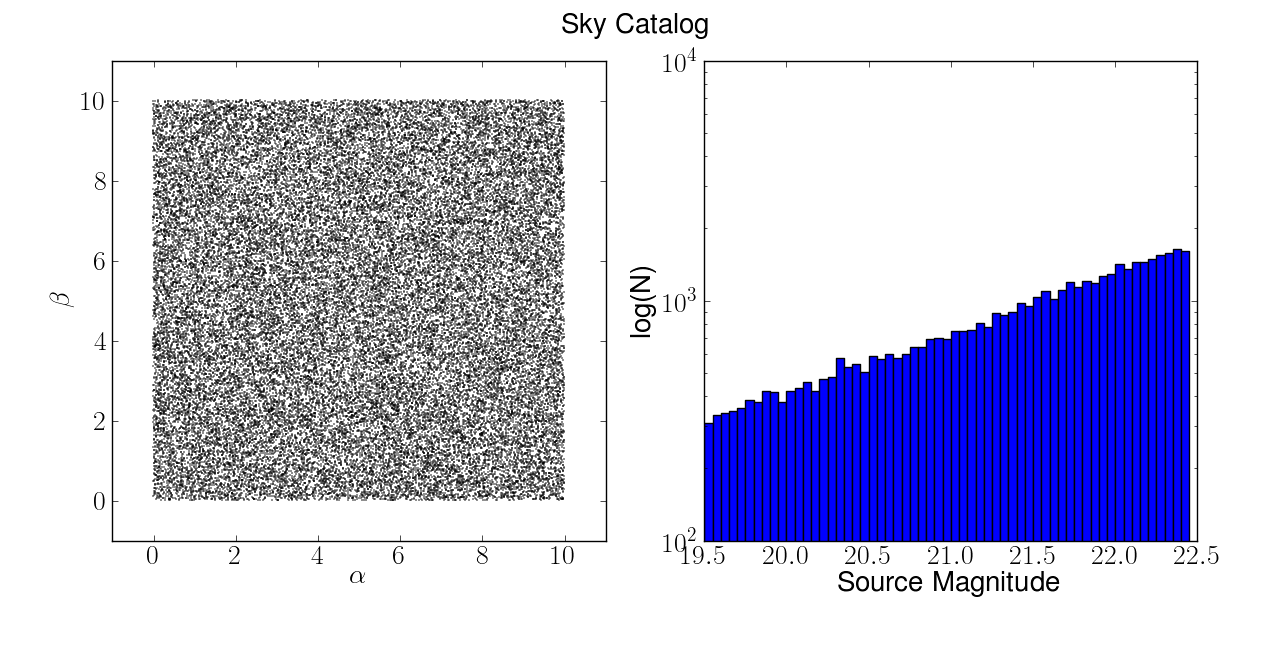
\includegraphics[width=\textwidth]{Catalog.png}
\end{center}
\caption{The catalog of fake stars. The stars are shown at their position on the sky (left) and as a histogram of their magnitudes (right).
\label{fig:sky}}
\end{figure}

We relate star magnitudes, $m$, to star fluxes, $s$, simply by:
\begin{displaymath}
m = 22.5 - 2.5\log_{10}(s)
\end{displaymath}
and therefore do not consider the NISP instrument's absolute response.

\section{Single Exposure}
With a given camera pointing $(\alpha, \beta)$ and camera orientation $(\theta)$, we transform the sky catalog into focal plane coordinates and find all the stars falling within the instrument's field-of-view. The NISP instrument's field-of-view of $0.7 \times 0.7$~deg$^{2}$ is used as the default in the simulations. We do not simulate images, instead we trivially convert the actual star fluxes into measured counts $(c)$ with a flat field model $(ff)$ and a noise model. A typical exposure is depicted in Figure \ref{fig:camera}.

\begin{figure}[ht]
\begin{center}
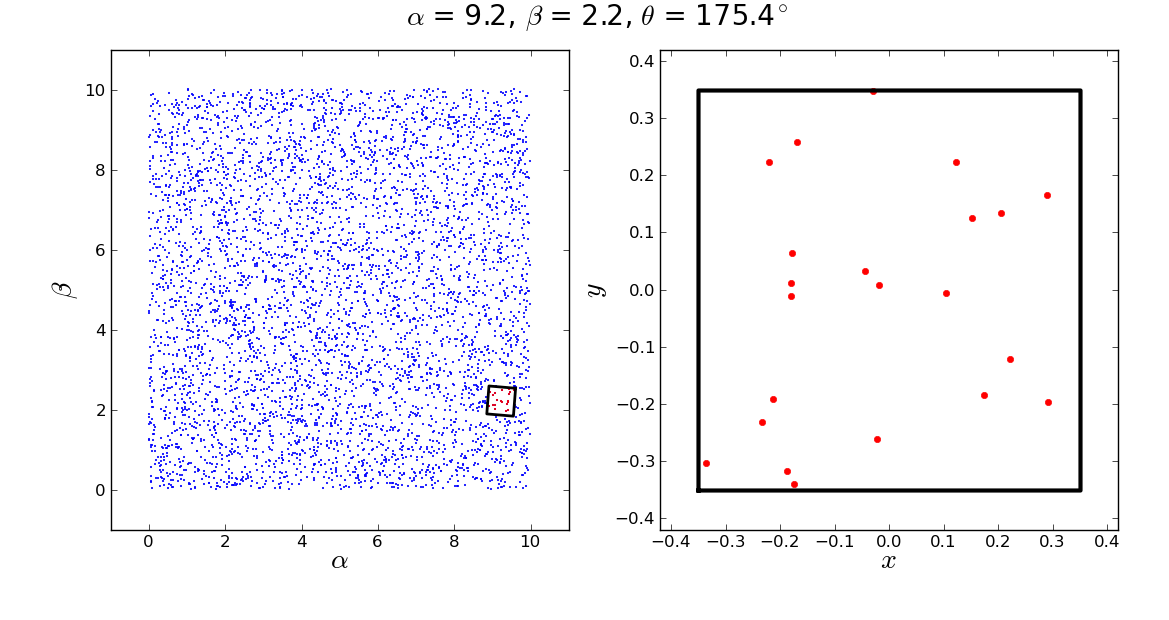
\includegraphics[width=\textwidth]{camera_image.png}
\end{center}
\caption{A single exposure of the sky with the pointing coordinates $(\alpha = 9.2^\circ, \beta = 2.2^\circ)$ and an orientation of $\theta = 175.4^\circ$. Left: Plot of the entire fake sky, with the instrument's field-of-view shown in black and the measured sources highlighted in red. Right: The distribution of the highlighted sources on the instrument's focal plane. \label{fig:camera}}
\end{figure}

\subsection{Uncertainty Variance}
We assume that the Euclid exposures will be background limited and that we will hit an upper limit on the signal-to-noise for bright sources. We model the uncertainty on the flux as:

\begin{displaymath}
\sigma_{{f}}^{2} = \alpha^{2} + \eta^{2} f^{2} 
\end{displaymath}

\noindent{}where $\alpha$ and $\eta$ are both constants (see Fig. \ref{fig:flux_uncertainty}).

\begin{figure}[ht]
\begin{center}
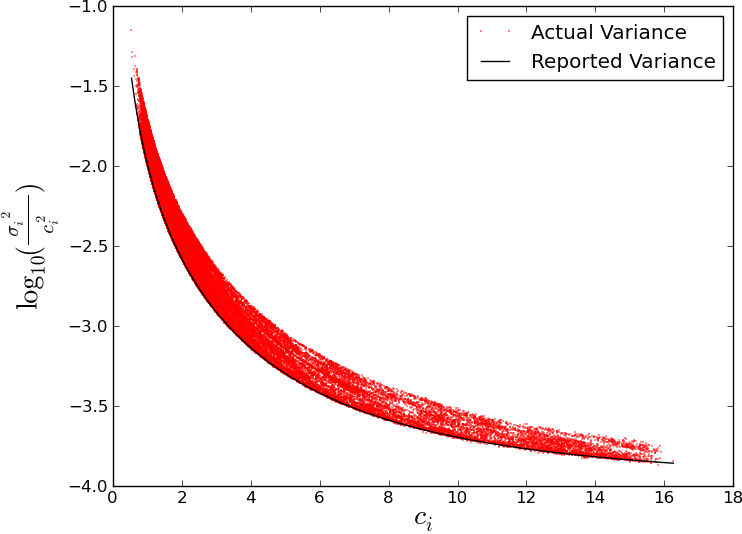
\includegraphics[width=\textwidth]{invvar_plot.png}
\end{center}
\caption{The flux uncertainty used as a function of star magnitude.\label{fig:flux_uncertainty}}
\end{figure}

\subsection{Catalog to Measured Flux Conversion}
The measured flux from a star depends on its focal plane position ($\vec{x_i}$), God's flat-field (with parameters $\vec{q}$) and the star's true flux ($s$). 

\begin{displaymath}
c_i = f(\vec{x_i} | \vec{q}) . s_{k} + e_{i}
\end{displaymath}

\noindent{}An error, drawn from the Normal Distribution $e_{ij} = N(e|0,{\sigma_i}^2)$, is also introduced to the measurement.



\end{document}
